\documentclass[aspectratio=169,11pt,t]{beamer}
% ============================================================
%  ksa-cs-v2: ksa-cs-lecture-template.tex 스타일 + 한글, v2 덱(16:9)용.
%    - 짙은 네이비 헤드라인 (섹션 이름 + 프레임마다 점)
%    - 꽉 찬 파란 제목 막대, 둥근 그림자 블록
%    - 한글: Noto Sans CJK KR (fontspec)
%  사용:
%    \documentclass[aspectratio=169,11pt,t]{beamer}
%    \input{<..>/theme/ksa-cs-v2.tex}
%  ksa-theme.tex 의 매크로(\kb \kq, ksablue/ksared 등)도 같은 이름으로 둔다
%  -> v2 덱 본문을 거의 그대로 옮길 수 있다.
% ============================================================

\usepackage{fontspec}
\usepackage{amsmath,amssymb}
\usepackage{tikz}
\usepackage{listings}
\usepackage{graphicx}
\usepackage{booktabs}
\usepackage{varwidth}
% enumitem 은 넣지 않는다 (beamer 글머리표가 사라진다)

\defaultfontfeatures{Ligatures=TeX}
\setmainfont{Noto Sans CJK KR}
\setsansfont{Noto Sans CJK KR}
\setmonofont{Noto Sans Mono CJK KR}[Scale=0.92]
\usefonttheme{professionalfonts}

% ---------- 기본 틀 ----------
\usetheme{default}
\useinnertheme[shadow=true]{rounded}
\setbeamertemplate{navigation symbols}{}
\setbeamersize{text margin left=1em,text margin right=1em}

% ---------- 색 (템플릿 원본 값) ----------
\definecolor{navydark}{HTML}{191959}
\definecolor{navydim}{HTML}{8888B0}
\definecolor{navytitle}{HTML}{262686}
\definecolor{navyblue}{HTML}{3333B2}
\definecolor{blockbodybg}{HTML}{E9E9F3}
\definecolor{examplegreen}{HTML}{006000}
\definecolor{examplebg}{HTML}{E5EFE5}
\definecolor{alertred}{HTML}{BF0000}
\definecolor{alertbg}{HTML}{F9E5E5}
% ksa-theme.tex 와 같은 이름 (본문 호환)
\colorlet{ksablue}{navytitle}
\colorlet{ksabluedk}{navydark}
\definecolor{ksagold}{HTML}{D6CBB1}
\definecolor{ksagolddk}{HTML}{A9976B}
\colorlet{ksared}{alertred}
\definecolor{ksagray}{HTML}{5B5B5B}

\setbeamercolor{structure}{fg=navyblue}
\setbeamercolor{alerted text}{fg=alertred}
\setbeamercolor{frametitle}{bg=navytitle,fg=white}
\setbeamercolor{title}{fg=white,bg=navytitle}
\setbeamercolor{block title}{bg=navytitle,fg=white}
\setbeamercolor{block body}{bg=blockbodybg,fg=black}
\setbeamercolor{block title example}{bg=examplegreen,fg=white}
\setbeamercolor{block body example}{bg=examplebg,fg=black}
\setbeamercolor{block title alerted}{bg=alertred,fg=white}
\setbeamercolor{block body alerted}{bg=alertbg,fg=black}
\setbeamercolor{item}{fg=navyblue}
\setbeamertemplate{itemize item}[circle]
\setbeamertemplate{itemize subitem}[triangle]

% ---------- 헤드라인: miniframes (섹션 이름 + 점) ----------
\useoutertheme[subsection=false]{miniframes}
\setbeamerfont{section in head/foot}{size=\tiny}
\setbeamercolor{section in head/foot}{bg=navydark,fg=white}
\setbeamercolor{mini frame}{fg=white}
\setbeamertemplate{mini frames}[circle]

% ---------- 제목 막대: 폭 꽉 채움, 두 줄까지 ----------
\setbeamerfont{frametitle}{size=\normalsize,series=\bfseries}
\setbeamertemplate{frametitle}{%
  \nointerlineskip
  \begin{beamercolorbox}[wd=\paperwidth,ht=2.7ex,dp=1.1ex,leftskip=.3cm,rightskip=.3cm]{frametitle}%
    \usebeamerfont{frametitle}\insertframetitle
  \end{beamercolorbox}}

% ---------- 쪽 번호: 오른쪽 아래 ----------
\setbeamertemplate{footline}{%
  \hfill
  {\color{navydim}\scriptsize\insertframenumber\,/\,\inserttotalframenumber}%
  \hspace{3mm}\vspace{2mm}%
}

% ---------- 표지: 템플릿처럼 헤드라인은 그대로, 가운데 둥근 그림자 상자에 제목 한 줄 ----------
% 덱에서:  {\setbeamertemplate{footline}{}\begin{frame}[c,noframenumbering]\titlepage\end{frame}}
\setbeamercolor{title}{fg=white,bg=navyblue}
\makeatletter
\setbeamertemplate{title page}{%
  \vfill
  \centering
  \begin{minipage}{0.84\paperwidth}
  \begin{beamercolorbox}[wd=\linewidth,sep=7pt,center,rounded=true,shadow=true]{title}
    {\usebeamerfont{title}\inserttitle\par}%
    \ifx\insertsubtitle\@empty\else\vskip0.4em{\usebeamerfont{subtitle}\insertsubtitle\par}\fi
  \end{beamercolorbox}
  \end{minipage}\par\vskip1.6em
  {\usebeamerfont{author}\color{navytitle}\insertauthor\par}\ifx\beamer@date\@empty\vskip0.3em\else\vskip1.3em\fi
  {\usebeamerfont{institute}\color{ksagray}\insertinstitute\par}%
  \ifx\beamer@date\@empty\else\vskip0.3em{\usebeamerfont{date}\color{ksagray}\insertdate\par}\fi
  \vfill
}
\makeatother
\setbeamerfont{title}{series=\bfseries,size=\Large}
\setbeamerfont{subtitle}{size=\normalsize}
\setbeamerfont{author}{size=\normalsize}
\setbeamerfont{institute}{size=\small}
\setbeamerfont{date}{size=\small}

% ksa-theme 호환: 덱이 \renewcommand{\ksacredit}{..} 를 해도 되게 (꼬리말에는 안 쓴다)
\newcommand{\ksacredit}{}

% ---------- 강조 ----------
\newcommand{\hl}[1]{\textcolor{alertred}{#1}}
\newcommand{\hlb}[1]{\textcolor{navyblue}{#1}}
\newcommand{\kb}[1]{\textbf{\color{ksablue}#1}}
\newcommand{\kq}[1]{\textbf{\color{ksared}#1}}

% ---------- 파이썬 코드 (템플릿과 같은 색) ----------
\definecolor{codekw}{HTML}{0033B3}
\definecolor{codebuiltin}{HTML}{BF0000}
\definecolor{codestr}{HTML}{067D17}
\definecolor{codecomment}{HTML}{8C8C8C}
\definecolor{codenum}{HTML}{1750EB}
\lstdefinestyle{py}{
  language=Python, basicstyle=\ttfamily\scriptsize,
  keywordstyle=\color{codekw}\bfseries, stringstyle=\color{codestr},
  commentstyle=\color{codecomment}\itshape, numberstyle=\color{codenum},
  emph={print,len,range,sum,input,int,str,float,list,dict,append,remove,sorted,abs,min,max},
  emphstyle=\color{codebuiltin}, showstringspaces=false, keepspaces=true,
  columns=fixed, basewidth=0.52em, aboveskip=1mm, belowskip=1mm, xleftmargin=2mm,
  breaklines=true
}
\lstset{style=py}

% 원본 덱 (ksa-theme) 의 그림·실습은 이 폴더로 합쳤다 (옛 원본: slides/old/v2/)
\setbeamerfont{author}{size=\normalsize}
\setbeamerfont{institute}{size=\small}
\graphicspath{{figs/}{../../../assets/}}
\makeatletter
\newcommand{\markpage}[1]{\protected@write\@auxout{}{\string\newlabel{#1}{{\the\c@framenumber}{}}}\hypertarget{#1}{}}
\newcommand{\pref}[1]{\hyperlink{#1}{\textcolor{ksagolddk}{(p.\ref{#1})}}}
\makeatother

\renewcommand{\ksacredit}{Machine Learning and Deep Learning \,\textperiodcentered\, kNN 최근접 이웃}
\title{kNN 최근접 이웃 (k-Nearest Neighbors)}
\subtitle{가장 가까운 k개에게 물어보기, 그리고 차원의 저주}
\author{Machine Learning and Deep Learning}
\institute{KSA 2027-Spring}
\date{Sumin Han (suminhan@ksa.hs.kr)}
\begin{document}
{\setbeamertemplate{footline}{}\begin{frame}[c,noframenumbering]\titlepage\end{frame}}

\section{질문}
% --- 오늘의 질문
\begin{frame}{오늘의 질문}
\vfill
\centering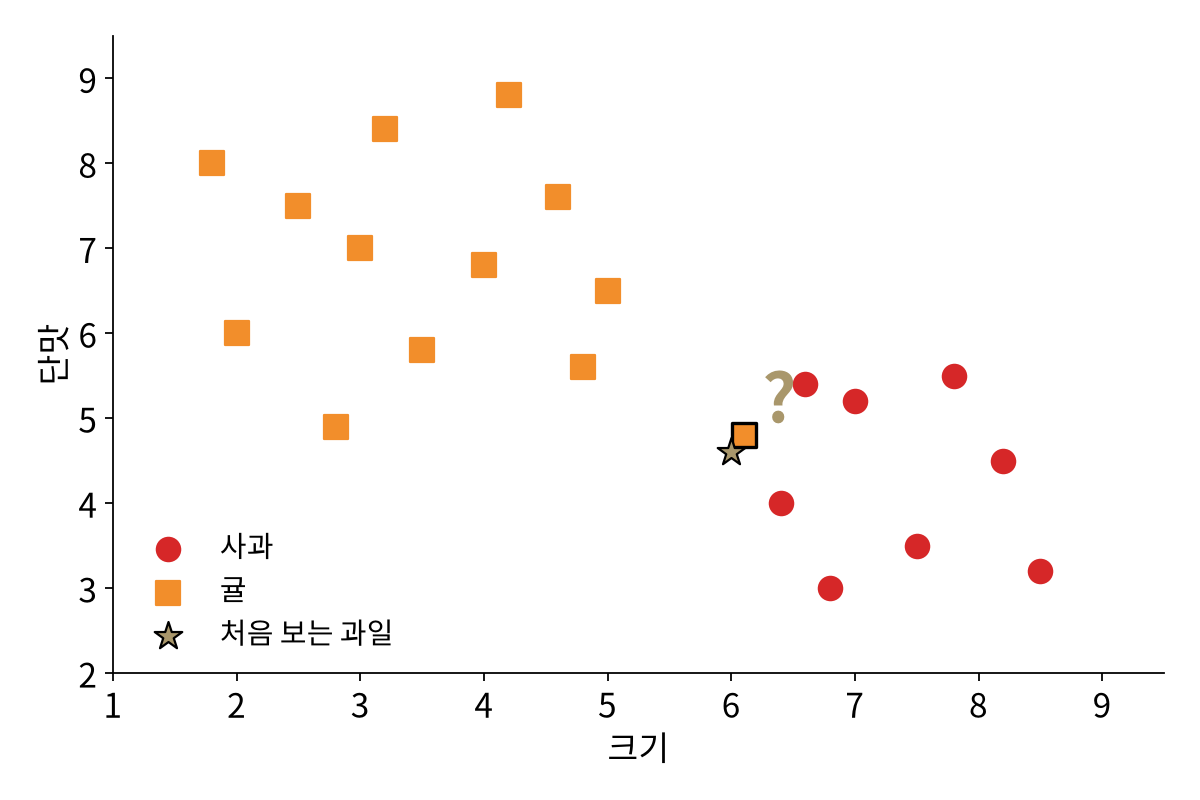
\includegraphics[width=0.56\linewidth]{kn_hook.png}\par\vskip0.2em
{\large 크기와 단맛을 잰 과일 21개. \kq{처음 보는 과일 (별) 은 사과일까, 귤일까?}}
\vfill
\note{과일 21개의 크기와 단맛을 재서 점으로 찍었습니다. 빨간 동그라미가 사과, 주황 네모가 귤입니다. 사과는 크고 덜 달고, 귤은 작고 더 답니다. 노란 별은 처음 보는 과일입니다. 사과일까요, 귤일까요? 공식을 몰라도 사람은 이렇게 답합니다. 주변에 사과가 많으니 사과겠지. 오늘 배울 kNN은 바로 이 생각을 그대로 알고리즘으로 만든 것입니다.}
\end{frame}

% --- 회귀와 분류
\begin{frame}{회귀 vs 분류 (regression vs classification)}
\vfill
\centering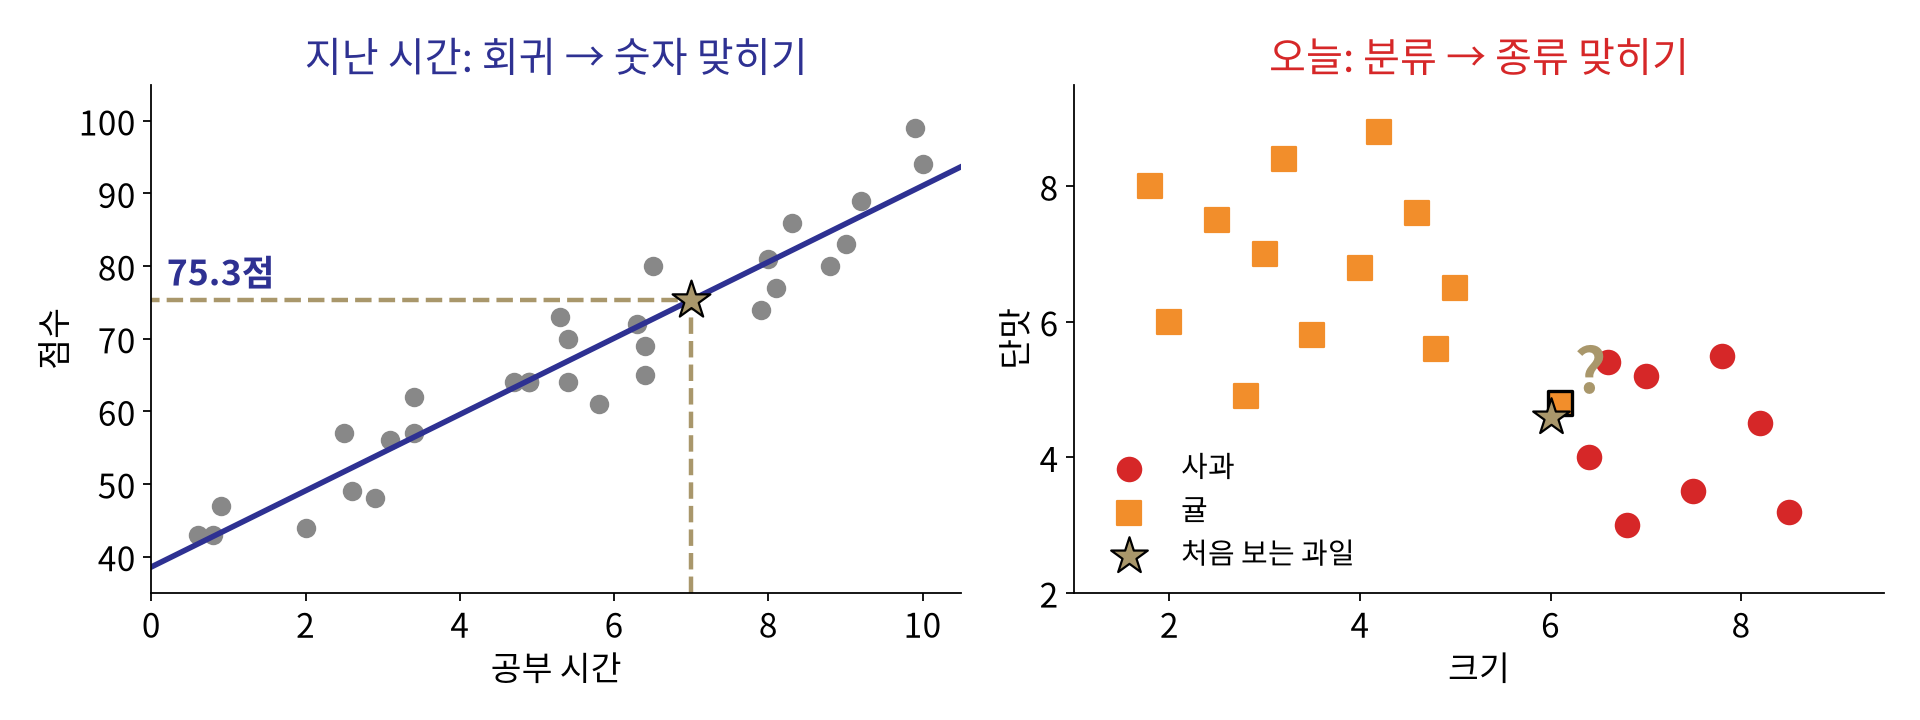
\includegraphics[width=0.88\linewidth]{kn_cls.png}\par\vskip0.4em
{\large \textbf{회귀}: 답이 \kb{숫자} (75.3 점) \qquad \textbf{분류}: 답이 \kq{종류} (사과 / 귤)}
\vfill
\note{지난 시간의 선형회귀는 답이 숫자였습니다. 공부 시간을 넣으면 점수가 나옵니다. 7시간이면 75.3점입니다. 이렇게 숫자를 맞히는 문제를 회귀라고 합니다. 오늘 문제는 답이 숫자가 아닙니다. 사과냐 귤이냐, 정해진 종류 중에서 하나를 고릅니다. 이런 문제를 분류라고 합니다. kNN은 분류를 가장 쉽게 보여 주는 대표적인 모델입니다. 선형회귀처럼 직선의 숫자를 배우지 않고, 데이터를 외워 두었다가 가까운 점들에게 묻습니다.}
\end{frame}

\section{이웃}
% --- k=3
\begin{frame}{가장 가까운 3개에게 묻기}
\markpage{k3}
\vfill
\begin{columns}[c]
\begin{column}{0.5\textwidth}\centering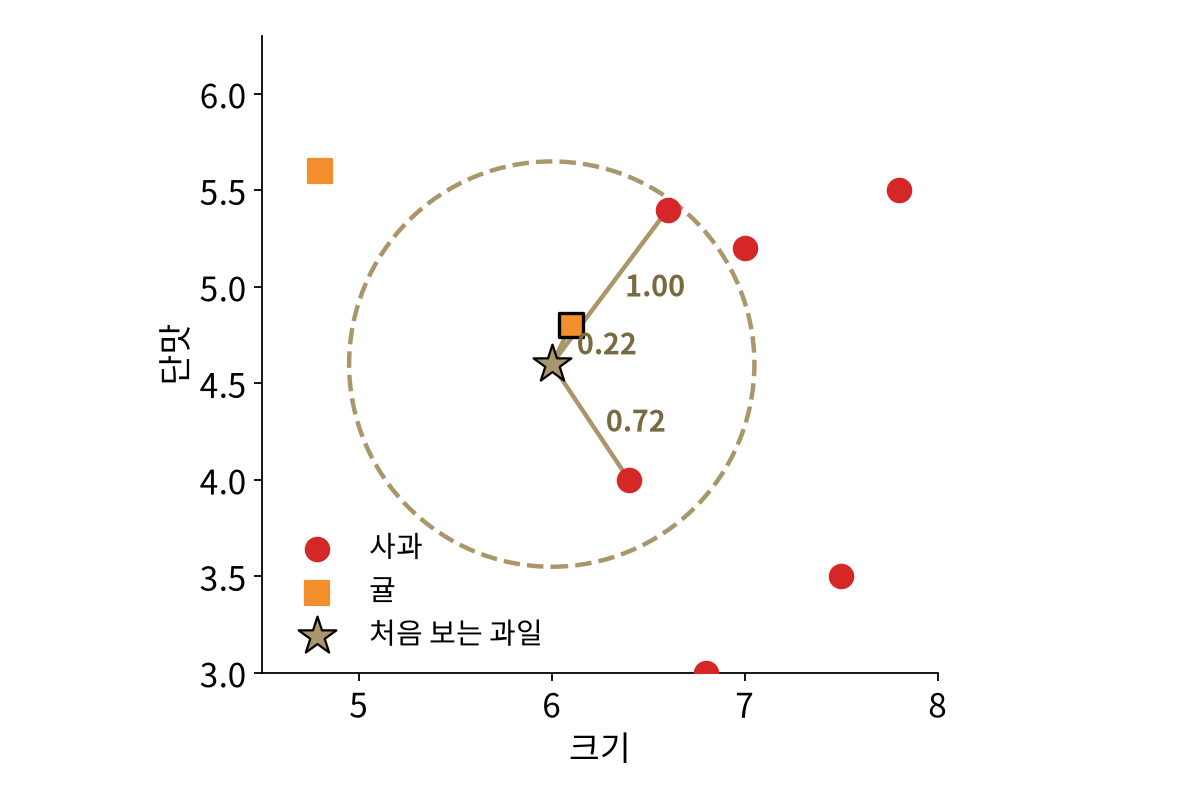
\includegraphics[width=\linewidth]{kn_k3.png}\end{column}
\begin{column}{0.46\textwidth}
{\large $k = 3$: 가장 가까운 3개}\\[0.6em]
{\large 귤 1 · 사과 2}\\[0.6em]
{\Large $\to$ 다수결로 \kq{사과}}\\[1em]
{\small kNN = k-Nearest Neighbors\\ (k-최근접 이웃)}
\end{column}
\end{columns}
\vfill
\note{별에서 가장 가까운 과일 3개를 찾습니다. 숫자는 별까지의 거리입니다. 0.22에 귤 하나, 0.72와 1.0에 사과 둘이 있습니다. 3개 중 사과가 2개이니 다수결로 사과라고 답합니다. 이것이 kNN, k 최근접 이웃의 전부입니다. k는 몇 개의 이웃에게 물어볼지를 정하는 숫자입니다.}
\end{frame}

% --- 거리
\begin{frame}{``가깝다'' = 유클리드 거리}
\vfill
\centering
{\LARGE\[ d(\mathbf{x}, \mathbf{q}) = \sqrt{\sum_{j=1}^{n} (x_j - q_j)^2} \]}\vskip0.4em
{\large 별 $(6.0,\ 4.6)$ 과 사과 $(6.4,\ 4.0)$: \quad $\sqrt{(6.4 - 6.0)^2 + (4.0 - 4.6)^2} = \sqrt{0.16 + 0.36} = 0.72$}\\[0.8em]
{\small $n$: 특징 수 (지금은 크기 · 단맛, 2개) \qquad 특징이 몇 개든 같은 식}
\vfill
\note{가깝다는 것은 보통 유클리드 거리, 즉 자로 잰 직선 거리입니다. 특징마다 차이를 제곱해서 더하고 루트를 씌웁니다. 별은 크기 6.0, 단맛 4.6이고, 가장 가까운 사과는 6.4와 4.0입니다. 차이는 0.4와 마이너스 0.6, 제곱하면 0.16과 0.36, 더하면 0.52, 루트를 씌우면 0.72입니다. 특징이 10개, 100개가 되어도 같은 식으로 잽니다. 이 점이 나중에 차원의 저주에서 문제가 됩니다.}
\end{frame}

% --- 학습 없음
\begin{frame}{학습이 없는 학습}
\vfill
\centering
\renewcommand{\arraystretch}{1.5}
{\large\begin{tabular}{rl}
\textbf{학습} & 데이터를 \kb{외워 두기만} 한다 \quad (가중치도, 경사하강법도 없다)\\
\textbf{예측} & \textcircled{1} 모든 점과 거리 재기 \; \textcircled{2} 가까운 순 정렬 \; \textcircled{3} 앞의 $k$ 개 다수결
\end{tabular}}\vskip1.0em
{\large 데이터 $m$ 개, 특징 $n$ 개 $\to$ 예측 한 번에 거리 계산 $m$ 번 (각각 $n$ 개 더하기)}\\[0.4em]
{\small 선형회귀는 학습이 느리고 예측이 빠르다. kNN 은 반대: \kq{비용이 예측할 때 몰린다}}
\vfill
\note{kNN에는 학습 단계가 사실상 없습니다. 선형회귀처럼 가중치를 찾지도, 경사하강법을 돌리지도 않습니다. 데이터를 외워 두기만 합니다. 대신 예측할 때마다 모든 점과 거리를 재고, 가까운 순으로 정렬해서, 앞의 k개로 다수결을 냅니다. 데이터가 m개면 예측 한 번에 거리를 m번 재야 합니다. 선형회귀는 학습이 오래 걸리지만 예측은 곱하기 몇 번이면 끝나는데, kNN은 반대로 비용이 예측 때 몰립니다. 데이터가 수백만 개면 이게 큰 문제가 되고, 그래서 가까운 점을 빨리 찾는 자료구조가 따로 연구됩니다.}
\end{frame}

% --- MNIST 에서 kNN 하는 법
\begin{frame}{손글씨 숫자 (MNIST): 그림 한 장 = 점 하나}
\vfill
\centering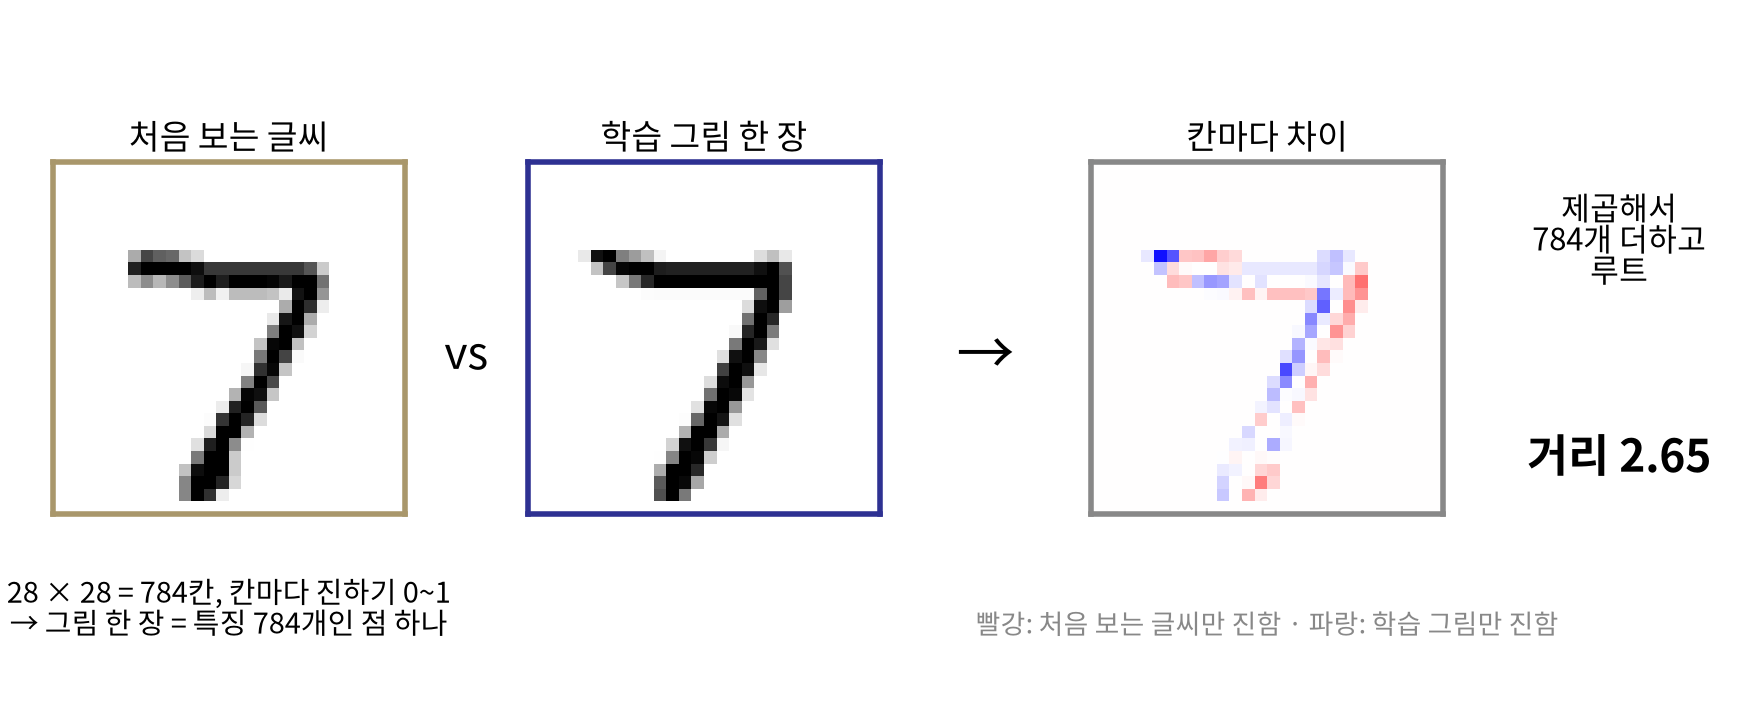
\includegraphics[width=0.9\linewidth]{kn_mnist_how.png}\par\vskip0.3em
{\large 과일과 같은 거리 식, 특징이 2개 $\to$ \kb{784개} \quad $d = \sqrt{\sum_{j=1}^{784}(x_j - x'_j)^2}$}
\vfill
\note{그럼 손글씨 숫자로 kNN을 하려면 어떻게 할까요. MNIST는 손으로 쓴 숫자 그림 7만 장, 학습 6만 장과 시험 1만 장입니다. 그림 한 장은 가로세로 28칸, 모두 784칸이고, 칸마다 진하기를 0에서 1로 나타냅니다. 이 784개 숫자를 한 줄로 늘어놓으면 그림 한 장이 특징 784개인 점 하나가 됩니다. 과일은 크기와 단맛, 특징 2개였는데 이번엔 784개일 뿐입니다. 두 그림의 거리도 같은 식입니다. 같은 자리 칸끼리 진하기 차이를 구하고, 제곱해서 784개를 다 더하고, 루트를 씌웁니다. 오른쪽 그림이 칸마다 차이입니다. 빨간 칸은 처음 보는 글씨에만 진하게 칠해진 곳, 파란 칸은 학습 그림에만 칠해진 곳이고, 둘 다 칠했거나 둘 다 비었으면 하얗게 0입니다. 획이 거의 겹치는 두 7이라 차이가 가장자리에만 조금 있고, 거리는 2.65입니다. 그다음은 과일과 똑같습니다. 학습 그림 6만 장 전부와 이 거리를 재고, 가장 가까운 k장의 숫자로 다수결을 냅니다. 픽셀은 모두 같은 0에서 1 눈금이라 따로 표준화하지 않습니다.}
\end{frame}

% --- 학습 없이 가장 가까운 한 장
\begin{frame}{학습 없이: 가장 가까운 한 장의 답을 그대로}
\vfill
\centering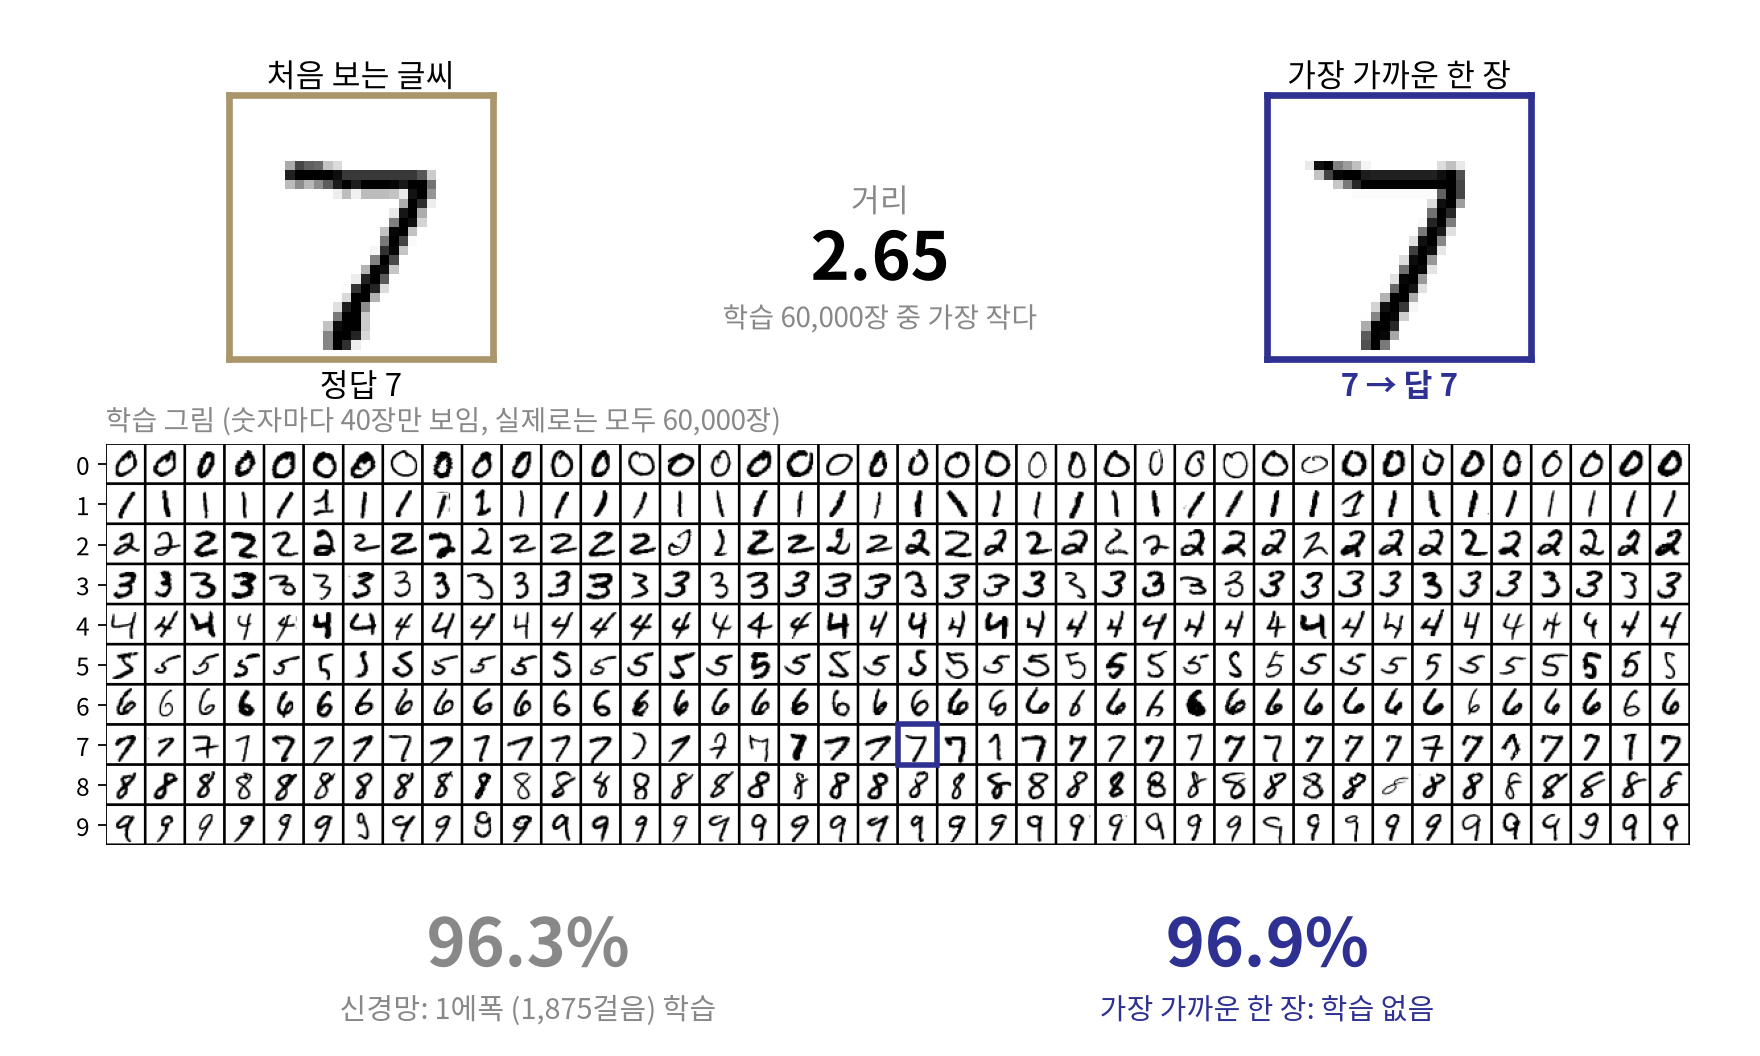
\includegraphics[width=0.66\linewidth]{kn_mnist_one.png}\par\vskip0.2em
{\large 시험 10,000장 중 \kb{9,691장} 맞힘 ($k = 1$) \quad 신경망 1에폭은 9,629장}
\vfill
\note{가장 단순하게, 가장 가까운 한 장, k가 1인 kNN을 해 봅시다. 처음 보는 7과 학습 6만 장 전부의 거리를 재면, 가장 가까운 것이 거리 2.65인 이 7이라 답은 7입니다. 가운데는 학습 그림을 숫자마다 40장씩만 보여 준 것이고, 파란 네모가 가장 가까운 그 한 장입니다. 실제로는 6만 장 전부와 잽니다. 시험 그림 1만 장에 모두 이렇게 하면 9,691장, 96.9퍼센트를 맞힙니다. 가중치도 없고 학습도 없이 외우기만 해서입니다. 비교로 은닉층 64개짜리 작은 신경망을 6만 장으로 한 바퀴, 1,875걸음 학습시키면 96.3퍼센트입니다. 다만 공정하게 말하면 신경망을 10바퀴 학습시키면 97.7퍼센트로 kNN을 넘고, 합성곱 신경망은 99퍼센트를 넘습니다. 그래도 학습 없이 이 정도라는 것은 놀랍습니다. 대신 kNN은 예측할 때마다 6만 장과 거리를 재야 합니다. 숫자는 exp_mnist.py 로 직접 잰 값입니다.}
\end{frame}

% --- 실제 데이터: 손글씨 숫자
\begin{frame}{가까운 $k$ 장의 다수결}
\vfill
\centering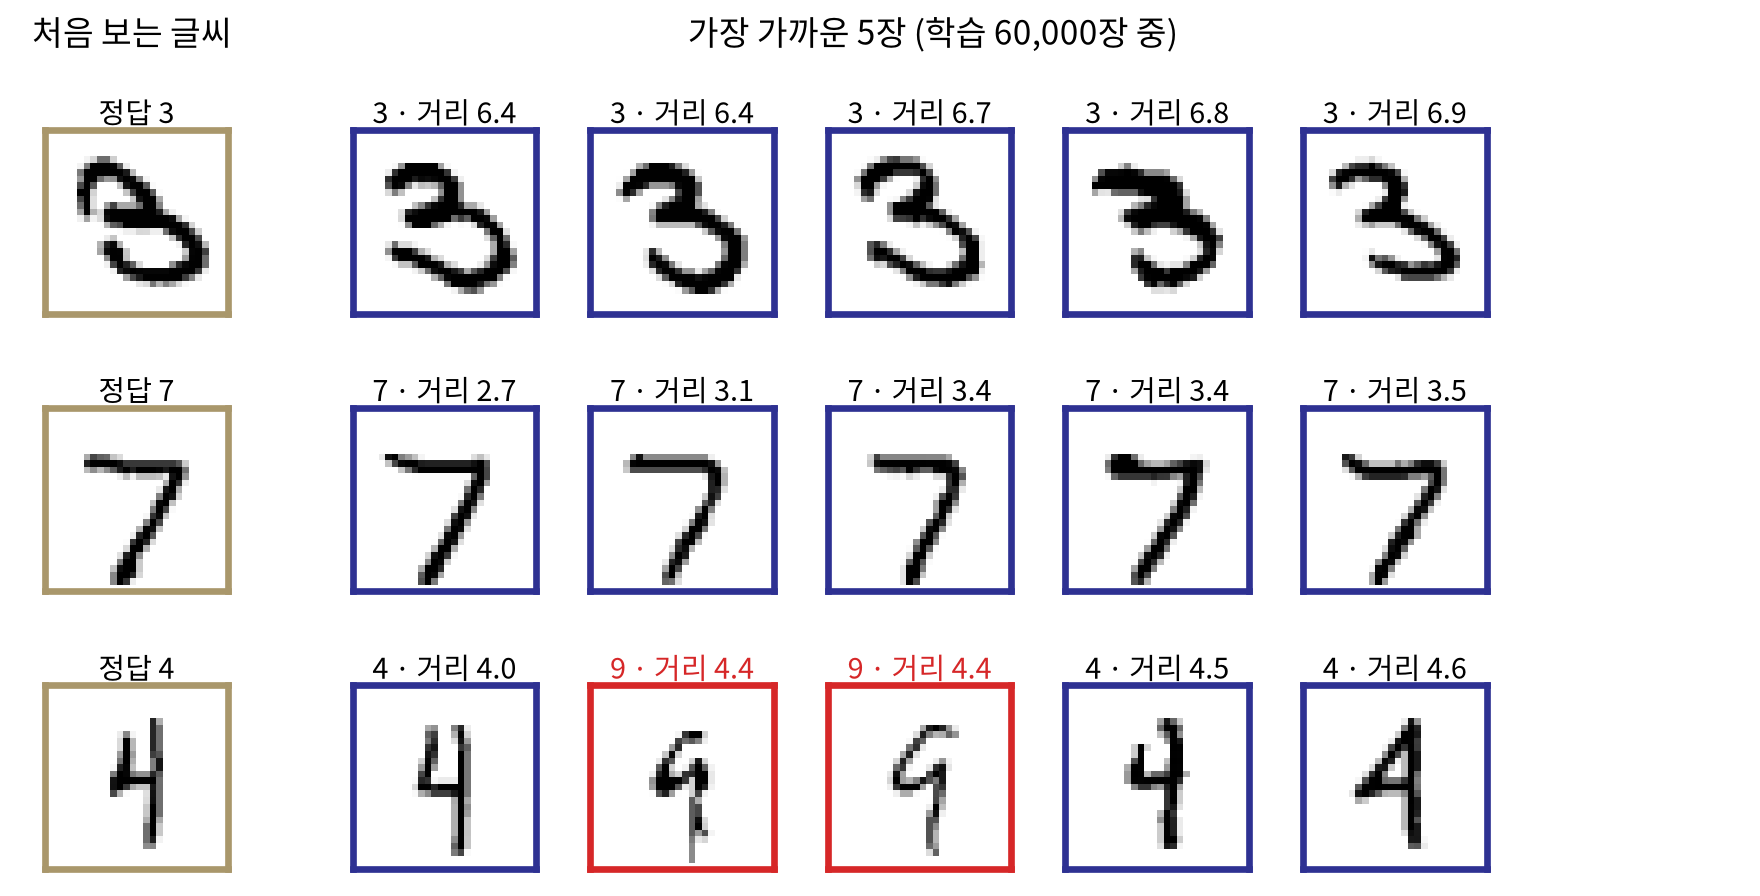
\includegraphics[width=0.64\linewidth]{kn_mnist.png}\par\vskip0.2em
{\large 가장 가까운 3장의 다수결 $\to$ 시험 정확도 \kb{97.2\%} \quad ($k = 1$ 은 96.9\%)}\\[0.2em]
{\small 마지막 줄: $k = 3$ 이면 9 (틀림), $k = 5$ 면 4 (맞힘)}
\vfill
\note{한 장 대신 가까운 몇 장의 다수결을 내 봅시다. 가장 가까운 3장의 다수결을 내면 97.2퍼센트를 맞혀, 한 장만 볼 때보다 조금 낫습니다. k가 1이면 96.9, 5면 96.9, 7이면 97.0퍼센트입니다. 첫 두 줄은 가까운 5장이 모두 같은 숫자라 쉽게 맞힙니다. 마지막 줄의 4는 위가 열린 4라서 9와 닮았습니다. 가장 가까운 3장이 4, 9, 9라 k가 3이면 9로 틀리고, 5장을 보면 4가 3장이라 맞힙니다. 다음 쪽에서 k를 어떻게 고르는지 봅니다. 숫자는 exp_mnist.py 로 직접 잰 값입니다.}
\end{frame}

\section{k 고르기}
% --- k 의 영향
\begin{frame}{$k$ 가 너무 작거나 너무 크면}
\markpage{boundary}
\vfill
\centering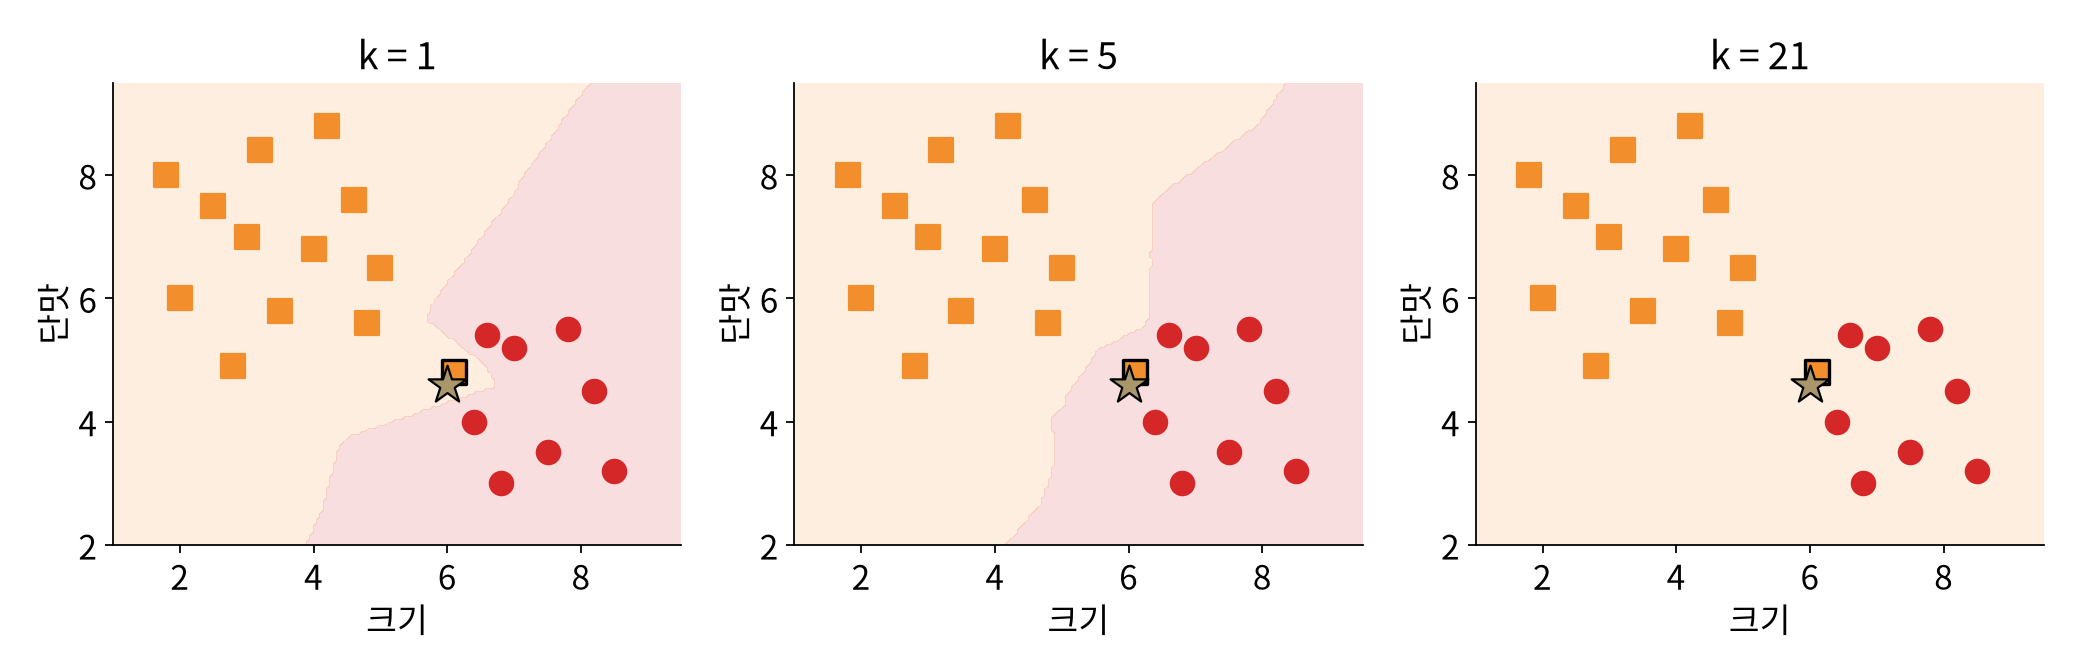
\includegraphics[width=0.96\linewidth]{kn_boundary.png}\par\vskip0.2em
{\large $k = 1$: 잘못 적힌 귤 (검은 테두리) 하나에 속는다 \quad $k = 21$: 전체 다수결 $\to$ \kq{늘 귤}}
\vfill
\note{배경색은 그 위치에 새 과일이 오면 어떻게 답할지를 칠한 것입니다. k가 1이면 가장 가까운 하나만 봅니다. 사과 무리 한가운데 귤로 잘못 적힌 점, 검은 테두리 네모가 있는데, 그 주변이 통째로 귤이 되어 버립니다. 별도 이 점 바로 옆이라 귤이라고 답합니다. 데이터의 실수까지 외우는 과대적합입니다. 반대로 k가 21, 전체 데이터면 언제나 전체의 다수결이니 귤 13개, 사과 8개로 어디서든 귤입니다. 너무 단순한 과소적합입니다. 가운데 k가 5일 때 경계가 가장 자연스럽습니다.}
\end{frame}

% --- k 고르기
\begin{frame}{$k$ 는 검증으로 고른다}
\vfill
\centering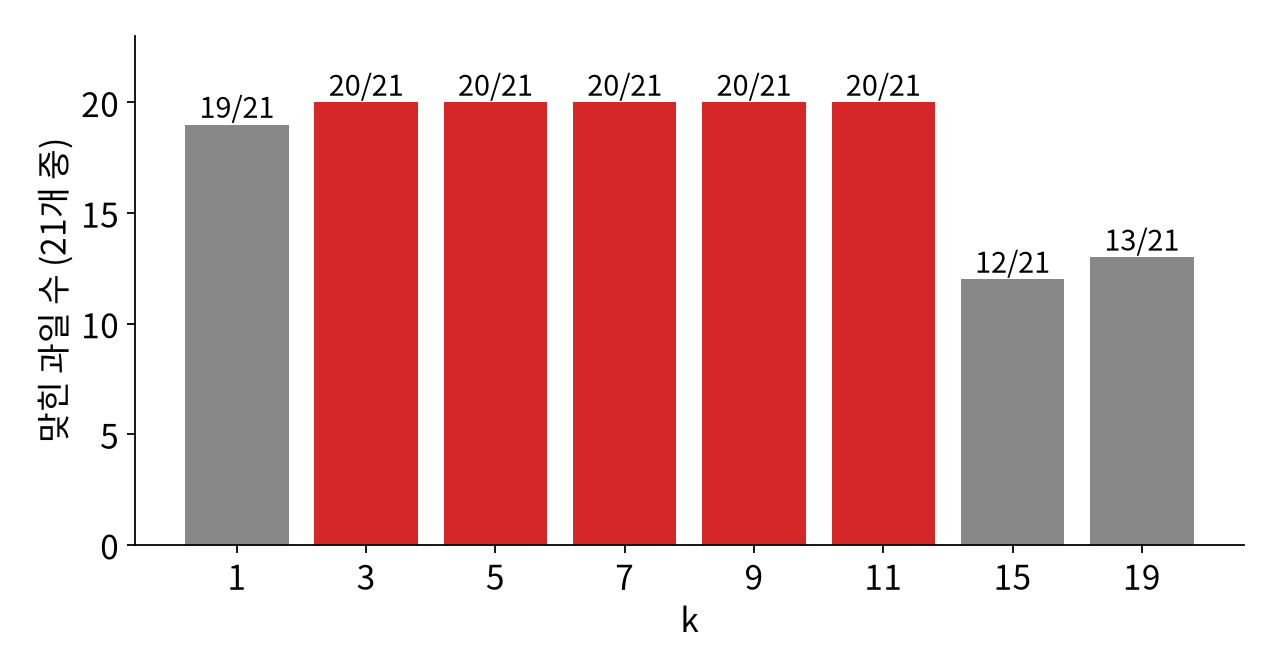
\includegraphics[width=0.56\linewidth]{kn_loo.png}\par\vskip0.2em
{\large 하나씩 빼 두고 나머지 20개로 맞혀 보기 \quad $k = 3 \sim 11$ 이 \kb{20/21}}\\[0.2em]
{\small \textbf{교차 검증} (cross-validation): 돌아가며 숨기고 맞히기 \; 하나씩 = leave-one-out}
\vfill
\note{그러면 k는 어떻게 고를까요? 교차 검증이라는 방법을 씁니다. 데이터 일부를 숨겨 두고 나머지로 맞혀 보는 일을 돌아가며 하는 것입니다. 데이터가 21개뿐이라 하나씩 숨겨 봅니다. 과일 하나를 빼 두고 나머지 20개로 kNN을 해서 맞히는지 보고, 21번 반복합니다. k가 1이면 21개 중 19개를 맞히는데, 3부터 11까지는 20개를 맞힙니다. 15를 넘으면 귤이 너무 많아져서 12개, 13개로 무너집니다. 이렇게 하나씩 빼는 교차 검증을 leave-one-out이라고 합니다. 동점이면 보통 작은 k가 계산이 빠르고, 이진 분류에서는 동점 투표가 안 나오게 홀수를 씁니다.}
\end{frame}

\section{표준화}
% --- 단위
\begin{frame}{단맛을 100 점 만점으로 재면?}
\markpage{scale}
\vfill
\centering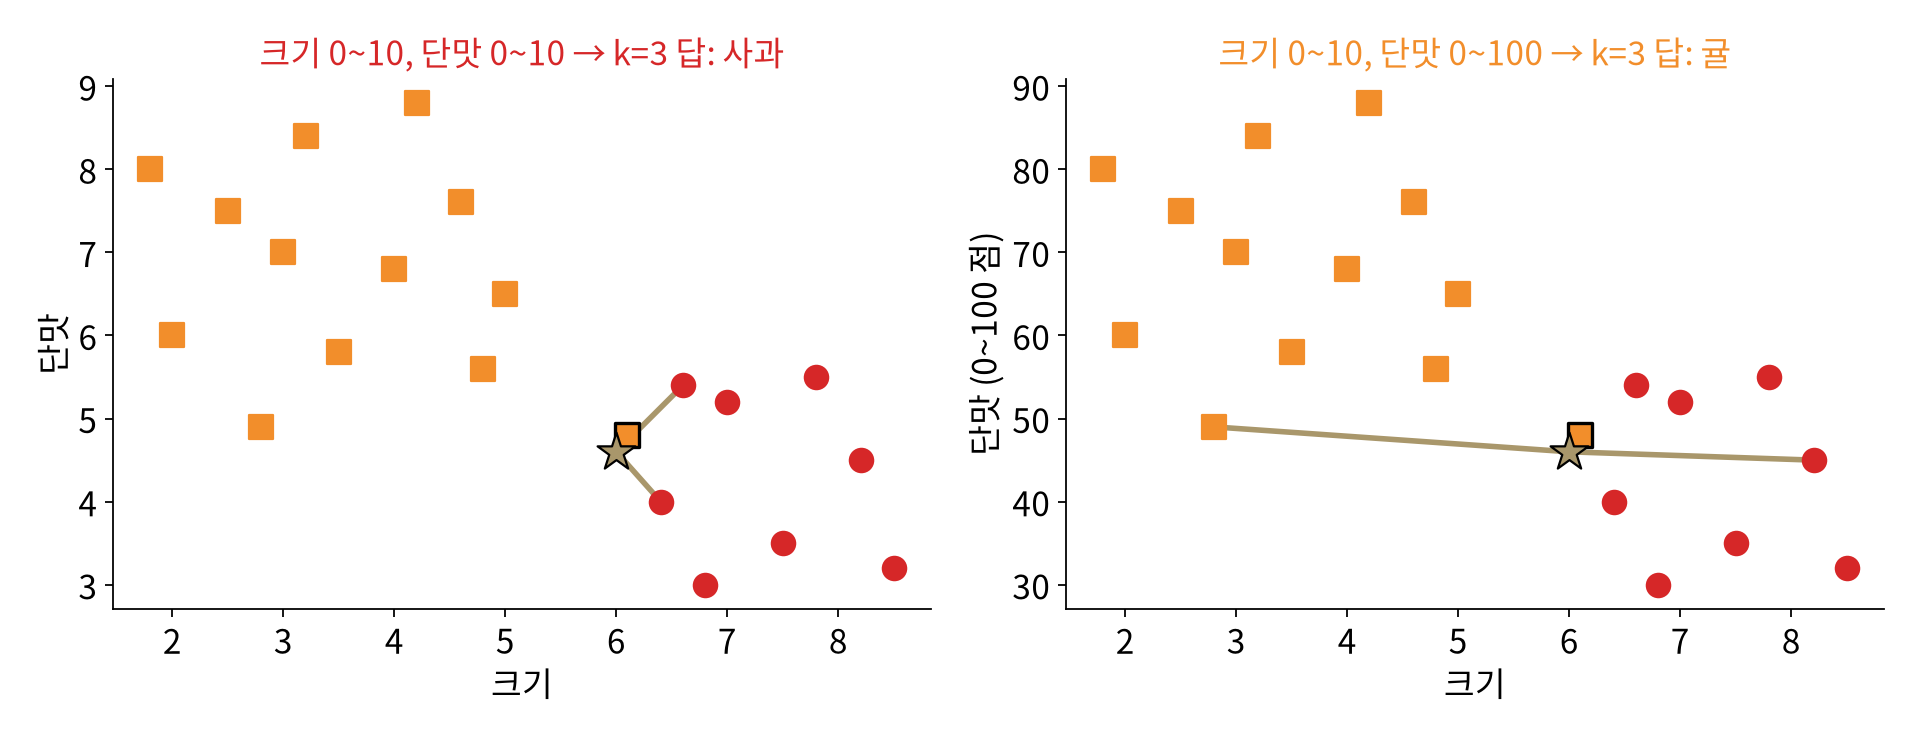
\includegraphics[width=0.86\linewidth]{kn_scale.png}\par\vskip0.2em
{\large 단위만 바꿨는데 $k = 3$ 의 답이 \kq{귤}로 \quad 거리를 \textbf{단맛}이 혼자 정한다}
\vfill
\note{단맛을 0에서 10이 아니라 100점 만점으로 재면 어떻게 될까요? 과일은 똑같고 단위만 바꿨습니다. 그런데 이제 단맛 차이는 10배가 되어서 거리를 거의 혼자 정합니다. 크기 차이는 무시되고, 단맛이 비슷한 과일만 가깝게 보입니다. 그 결과 k가 3일 때 가까운 이웃이 귤 둘, 사과 하나로 바뀌고 답이 귤이 됩니다. 단위를 바꿨을 뿐인데 답이 바뀐 겁니다.}
\end{frame}

% --- 표준화
\begin{frame}{해결: 특징마다 같은 목소리 (표준화)}
\vfill
\centering
{\LARGE\[ z_j = \frac{x_j - \mu_j}{\sigma_j} \]}\vskip0.4em
{\large 특징마다 평균 0, 표준편차 1 로 맞춘 뒤 거리를 잰다 \quad (표준점수 $z$)}\\[0.8em]
{\large 실제 데이터 (와인 178병, 특징 13개): \; 그대로 \textbf{71\%} \quad 표준화 후 \kb{97\%} \quad ($k = 5$)}\\[0.4em]
{\small 와인 데이터에서 프롤린은 수백 $\sim$ 1,600, 색 농도는 1 $\sim$ 13 $\to$ 그대로 두면 프롤린 하나가 거리를 정한다}
\vfill
\note{해결책은 표준화입니다. 특징마다 평균을 빼고 표준편차로 나눠서, 모든 특징을 평균 0, 표준편차 1로 맞춥니다. 이렇게 바꾼 값을 표준점수, z 점수라고 부릅니다. 그러면 단위와 상관없이 모든 특징이 같은 크기의 목소리를 냅니다. 실습에서 쓸 와인 데이터는 와인 178병의 화학 성분 13개로 품종 셋을 맞히는 문제입니다. 그대로 kNN을 하면 71퍼센트인데, 표준화하면 97퍼센트가 됩니다. 프롤린이라는 성분은 수백에서 1600까지인데 다른 성분은 1에서 13 정도라서, 그대로 두면 프롤린 하나가 거리를 정해 버리기 때문입니다.}
\end{frame}

\section{차원의 저주}
% --- 차원의 저주 1
\begin{frame}{차원의 저주: 가까운 이웃이 사라진다}
\vfill
\centering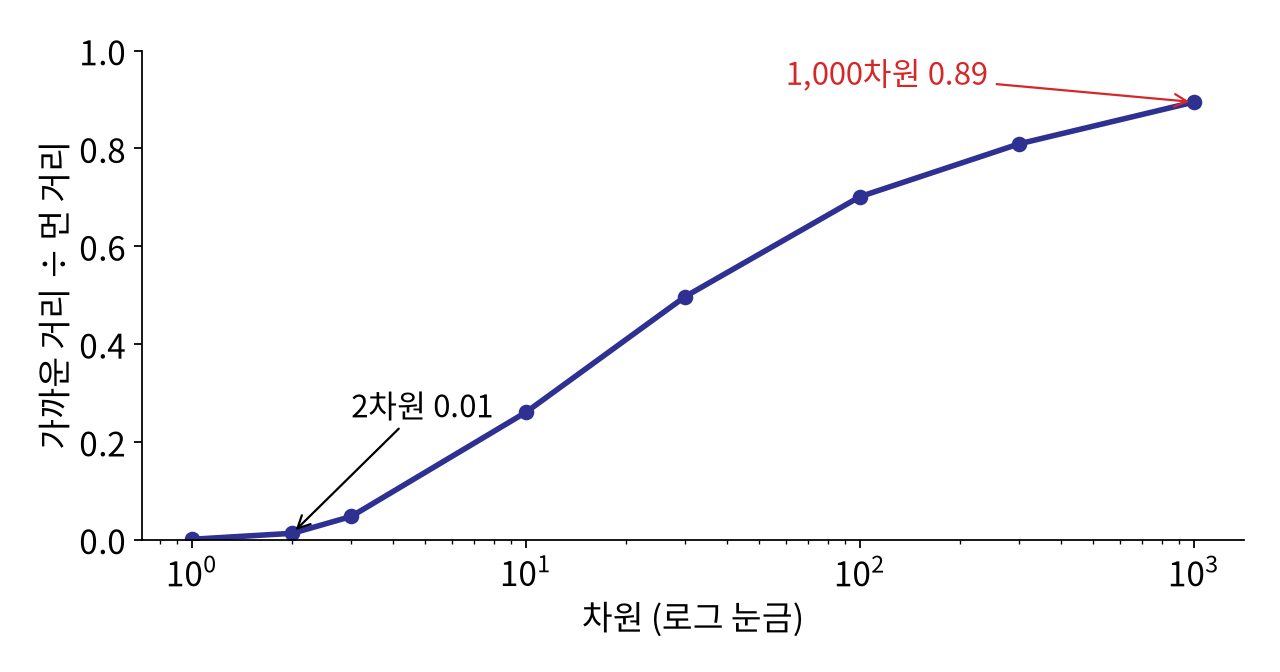
\includegraphics[width=0.56\linewidth]{kn_ratio.png}\par\vskip0.2em
{\large 가장 가까운 거리 $\div$ 가장 먼 거리 (점 1,000개): \quad 2차원 \kb{0.01} $\to$ 1,000차원 \kq{0.9}}\\[0.2em]
{\small 차원이 높으면 가장 가까운 점도 가장 먼 점만큼 멀다 \quad Curse of Dimensionality (Bellman, 1957)}
\vfill
\note{특징이 많아지면 kNN에는 더 근본적인 문제가 생깁니다. 정육면체 안에 점 1000개를 균등하게 뿌리고, 한 점에서 가장 가까운 점까지의 거리를 가장 먼 점까지의 거리로 나눠 봤습니다. 2차원에서는 0.01, 가까운 점은 정말 가깝습니다. 그런데 차원을 올릴수록 이 비율이 1에 가까워져서 1000차원에서는 0.9입니다. 가장 가까운 점도 가장 먼 점과 거의 같은 거리에 있다는 뜻입니다. 그러면 가장 가까운 이웃이라는 말 자체가 의미를 잃습니다. 이 현상을 차원의 저주라고 하고, 1957년 벨만이 붙인 이름입니다.}
\end{frame}

% --- 차원의 저주 2
\begin{frame}{뜻 없는 특징을 더하면}
\vfill
\centering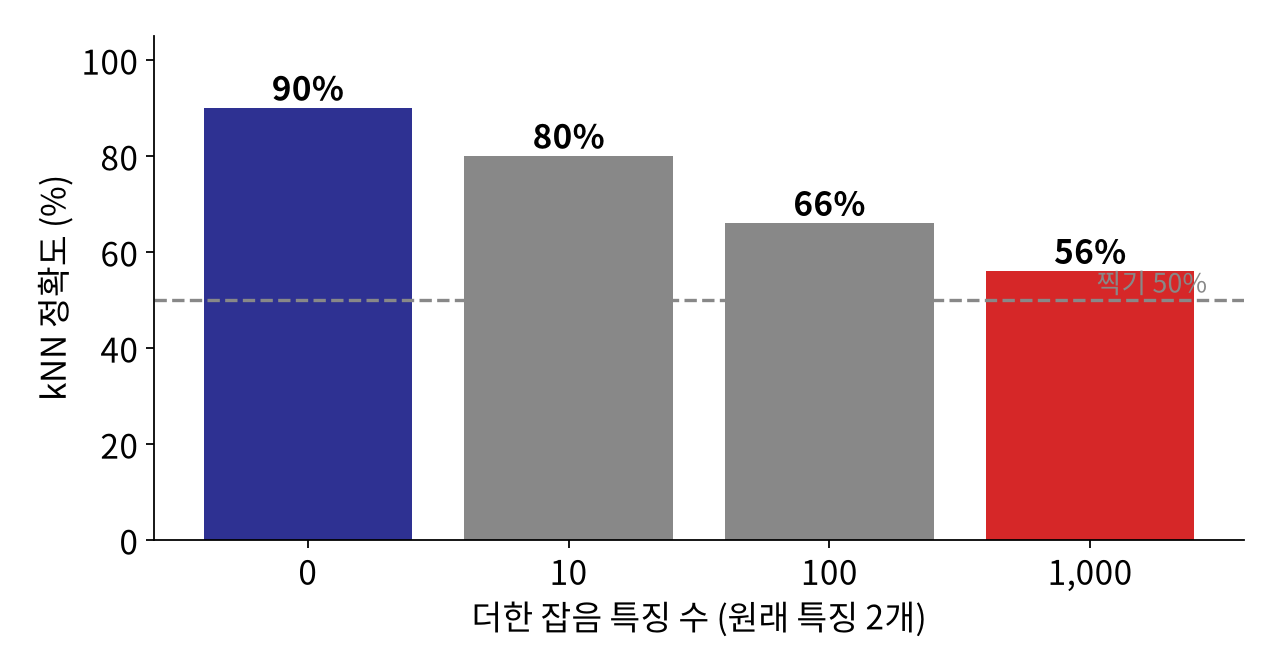
\includegraphics[width=0.56\linewidth]{kn_noise.png}\par\vskip0.2em
{\large 두 반달 데이터 (특징 2개) 에 난수 특징을 더하면 \quad 90\% $\to$ 80 $\to$ 66 $\to$ \kq{56\%}}\\[0.2em]
{\small 특징은 많을수록 좋은 게 아니다 $\to$ 쓸모 있는 특징만 고르거나, 차원을 줄인다 (6주차 PCA)}
\vfill
\note{실제로 얼마나 나빠질까요? 두 반달 모양으로 나뉜 데이터는 특징 2개만으로 kNN 정확도가 90퍼센트입니다. 여기에 아무 뜻 없는 난수 특징을 10개 더하면 80퍼센트, 100개면 66퍼센트, 1000개면 56퍼센트로 거의 찍기 수준이 됩니다. 원래의 유용한 두 특징은 그대로 있는데도요. 뜻 없는 축의 거리가 쌓여서 진짜 차이를 덮어 버리기 때문입니다. 그래서 특징은 많을수록 좋은 게 아닙니다. 쓸모 있는 특징만 고르거나, 6주차에 배울 PCA처럼 차원을 줄인 뒤에 거리를 잽니다.}
\end{frame}

\section{연습}
% --- 문제풀이
\begin{frame}{문제풀이}
\vfill
\begin{enumerate}
\item 점 A $(1, 1)$ 사과, B $(2, 3)$ 귤, C $(4, 1)$ 사과, D $(3, 4)$ 귤. 새 점 $(2, 2)$ 에 대해 (a) 네 거리는? \; (b) $k = 1$, $k = 3$ 의 답은?\vskip0.8em
\item 학습 데이터 100만 개로 kNN 과 선형회귀를 만들었다. 예측 한 번이 더 오래 걸리는 쪽은? 이유는?\vskip0.8em
\item 키 (cm) 와 몸무게 (kg) 로 kNN 을 한다. 키를 mm 로 바꾸면 무슨 일이 생기나? 어떻게 막나?\vskip0.8em
\item 특징 2개로 90\% 이던 kNN 에 특징을 50개 더했더니 70\% 가 됐다. 무엇을 의심해야 하나?
\end{enumerate}
\vfill
\note{1번 답. A까지 루트 2, 약 1.41, B까지 1, C까지 루트 5, 약 2.24, D까지 루트 5, 약 2.24입니다. k가 1이면 가장 가까운 B, 귤입니다. k가 3이면 B와 A, 그리고 C와 D가 같은 거리라서 동점입니다. 동점 처리 규칙이 필요하다는 게 답의 핵심이고, 예를 들어 먼저 나온 C를 쓰면 사과 2, 귤 1로 사과입니다. 2번 답. kNN입니다. 예측할 때마다 100만 개와 거리를 재야 하니까요. 3번 답. 키 차이가 10배가 되어 거리를 키가 혼자 정합니다. 표준화로 막습니다. 4번 답. 차원의 저주입니다. 더한 특징이 쓸모없는 잡음일 가능성을 의심하고, 특징을 골라 봅니다.}
\end{frame}

% --- 실습
\begin{frame}{실습}
\vfill
\centering\begin{tabular}{rl}
\large 1 & kNN 직접 구현: 거리 · 정렬 · 다수결 $\to$ 슬라이드의 과일로 $k = 1, 3, 21$ 재현\\[0.5em]
\large 2 & 실제 데이터: 와인 178병, 표준화 전후 비교 (71\% $\to$ 97\%)\\[0.5em]
\large 3 & 교차 검증으로 $k$ 고르기 + 잡음 특징을 더하며 차원의 저주 보기
\end{tabular}\vskip1em
Wine (Forina et al.; UCI) \\[0.4em]\href{https://colab.research.google.com/github/SuminHan/book-ml/blob/main/slides/ml1/week01/3_knn/lab/knn.ipynb}{\textcolor{ksagolddk}{▶ Colab에서 실습 노트북 열기}}
\vfill
\note{실습은 세 부분입니다. 첫째, 거리 재기, 정렬, 다수결 세 단계를 직접 구현해서 슬라이드의 과일로 k가 1, 3, 21일 때 답을 재현합니다. 둘째, 실제 와인 데이터로 표준화를 하기 전과 후를 비교합니다. 셋째, 교차 검증으로 k를 고르고, 잡음 특징을 더해 가며 정확도가 어떻게 무너지는지 직접 봅니다.}
\end{frame}

\section{정리}
% --- 정리
\begin{frame}{정리}
\vfill
\centering\large\begin{tabular}{l}
\textbf{kNN} \quad 가장 가까운 $k$ 개의 다수결 \quad 학습 없이 외우고, 예측 때 거리를 잰다\\[0.5em]
$k$ 가 작으면 과대적합, 크면 과소적합 $\to$ \textbf{교차 검증}으로 고른다\\[0.5em]
단위가 다르면 거리가 왜곡된다 $\to$ \kb{표준화} 먼저\\[0.5em]
특징이 많으면 이웃이 사라진다 $\to$ \kq{차원의 저주}
\end{tabular}
\vfill
\note{정리합니다. kNN은 가장 가까운 k개의 다수결입니다. 학습 단계 없이 데이터를 외워 두고, 예측할 때마다 거리를 잽니다. k가 작으면 잡음까지 외우는 과대적합, 크면 늘 많은 쪽만 답하는 과소적합이라 교차 검증으로 고릅니다. 특징의 단위가 다르면 거리가 왜곡되니 표준화를 먼저 하고, 특징이 너무 많으면 차원의 저주로 가까운 이웃이라는 개념 자체가 무너집니다. 다음 시간에는 데이터에서 경계선을 학습하는 분류 방법, 로지스틱회귀를 배웁니다.}
\end{frame}
\end{document}
